\documentclass[12pt]{article}
\setlength\parindent{0pt}
\usepackage{amsmath}
\usepackage{lscape}
\usepackage{graphicx}
\usepackage{fullpage}
\usepackage[margin=0.8in]{geometry}
\setlength{\parskip}{4mm}
\def\LL{\left\langle}   % left angle bracket
\def\RR{\right\rangle}  % right angle bracket
\def\LP{\left(}         % left parenthesis
\def\RP{\right)}        % right parenthesis
\def\LB{\left\{}        % left curly bracket
\def\RB{\right\}}       % right curly bracket
\def\PAR#1#2{ {{\partial #1}\over{\partial #2}} }
\def\PARTWO#1#2{ {{\partial^2 #1}\over{\partial #2}^2} }
\def\PARTWOMIX#1#2#3{ {{\partial^2 #1}\over{\partial #2 \partial #3}} }
\newcommand{\BE}{\begin{displaymath}}
\newcommand{\EE}{\end{displaymath}}
\newcommand{\BI}{\begin{itemize}}
\newcommand{\EI}{\end{itemize}}
\newcommand{\BNE}{\begin{equation}}
\newcommand{\ENE}{\end{equation}}
\newcommand{\BEA}{\begin{eqnarray}}
\newcommand{\EEA}{\nonumber\end{eqnarray}}
\newcommand{\EL}{\nonumber\\}
\newcommand{\la}[1]{\label{#1}}
\newcommand{\ie}{{\em i.e.\ }}
\newcommand{\eg}{{\em e.\,g.\ }}
\newcommand{\cf}{cf.\ }
\newcommand{\etc}{etc.\ }
\newcommand{\Tr}{{\rm tr}}
\newcommand{\etal}{{\it et al.}}
\newcommand{\OL}[1]{\overline{#1}\ } % overline
\newcommand{\OLL}[1]{\overline{\overline{#1}}\ } % double overline
\newcommand{\OON}{\frac{1}{N}} % "one over N"
\newcommand{\OOX}[1]{\frac{1}{#1}} % "one over X"
\pagenumbering{gobble}
\begin{document}
\Large

\begin{center}
	\sc \Large Homework 4 Quiz-- Kepler's Laws (form 2)
	
	Name: \underline{\hspace{2in}} Lab Section: \underline{\hspace{2in}}
\end{center}
\normalsize





\begin{enumerate}
	\item Draw a moderately eccentric orbit around the star shown such that the point marked with an X is the point where the planet is the closest to its star.
	
	\vspace{2in}
	
	\begin{center}
	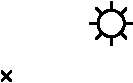
\includegraphics[width=0.16\textwidth]{quiz1-crop.pdf}
	\end{center}

	\vspace{2in}

\vfill

\begin{center}

(There is another question on the back of this page.)	

\end{center}

	\newpage
	
	\item Here is a diagram of the orbit of a moon around its planet. Suppose that the moon orbits the planet counterclockwise as seen from this perspective.
	
	The moon takes twelve Earth days to orbit its planet; its location each day is shown with a dot alongside the orbit.
	
	
	\begin{center}
		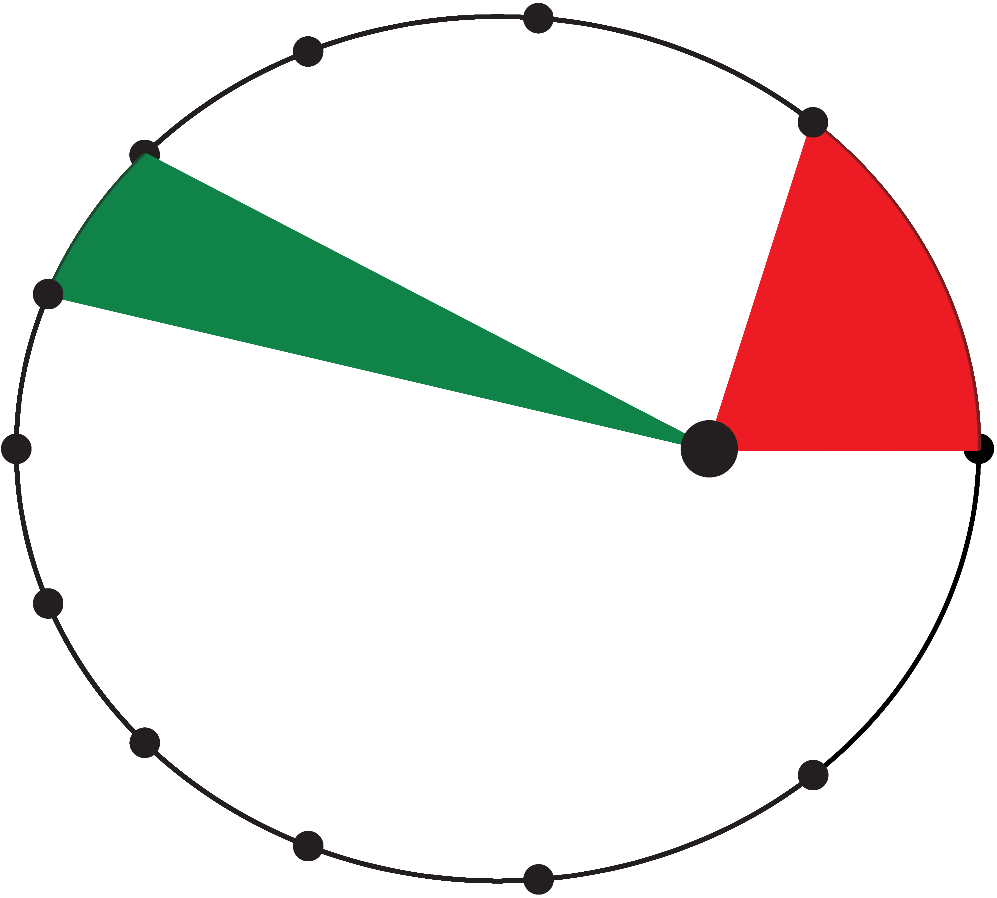
\includegraphics[width=0.5\textwidth]{quiz-two-crop.png}
	\end{center}
	
	\begin{enumerate}
		\item Choose a location where the planet is {\it slowing down} and label it (a)
		\item Find the location where the planet is {\it moving fastest} and label it (b)
		\item How does the {\it area} of the red shaded region on the right compare to the area of the green shaded region on the left? (Which one is larger, or are they equal?)
		
		\vspace{1in}
		
		\item Explain briefly how you know.
		
	\end{enumerate}


	\end{enumerate}

	
\end{document}




